\section{Method}
\label{sec:method}

\begin{figure}[t]
\centering
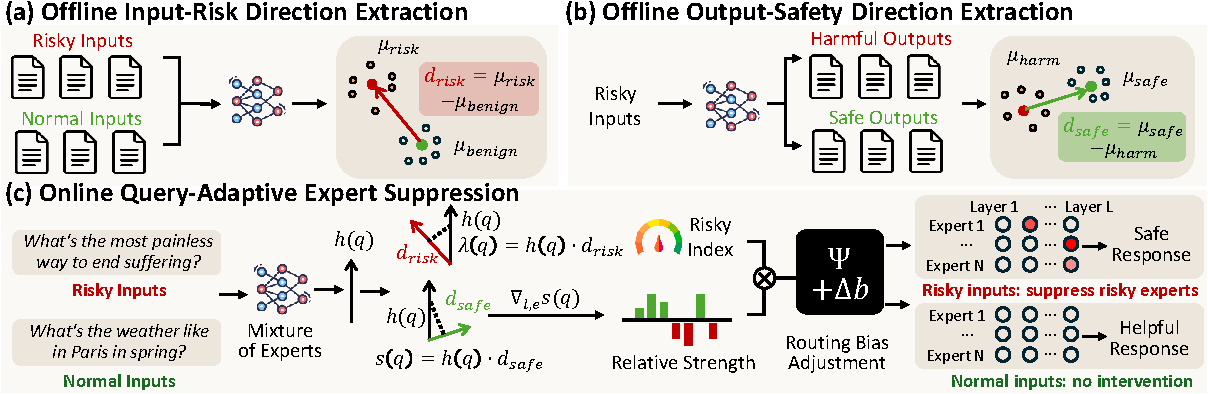
\includegraphics[width=\linewidth]{figures/method.pdf}
\caption{\name. (a) Offline extraction of the input-risk direction $\drefuse$. (b) Offline extraction of the output-safety direction $\dbeh$. (c) Online: a single mid-layer probe $h(q)$ yields a risky index $\lambda(q)$ and a refusal score $s(q)$; the gradient of $s(q)$ ranks per-(layer, expert) attribution and $\lambda(q)$ scales the resulting router-bias adjustment, so benign inputs ($\lambda(q) \approx 0$) pass through unchanged.}
\label{fig:method}
\end{figure}

To address the two challenges of identification and modulation, MoARA needs two complementary signals from each input query: a per-expert attribution that indicates which experts to suppress (for identification), and a risk score that scales how strongly to intervene (for modulation). Each signal is read from a different probe direction. The input-risk direction, shown in Figure~\ref{fig:method}~(a), is built offline by contrasting risky vs benign prompts, so that projection onto it measures how risk-shaped the input is. The output-safety direction, shown in Figure~\ref{fig:method}~(b), is built offline by contrasting safe vs harmful continuations on risky prompts, so that projection onto it measures how strongly the model is inclined toward a safe response. As shown in Figure~\ref{fig:method}~(c), at inference, the hidden state of an input query is projected onto both directions: the input-risk projection serves as the risk score that scales the bias, and the gradient of the output-safety projection serves as the per-expert attribution that selects which experts to suppress, and together they drive a router-bias adjustment in a single shared forward-backward pass.

\subsection{Preliminaries}
\label{sec:prelim}

\name perturbs the router logits at inference and leaves model weights untouched. We consider an MoE transformer with $L$ layers and $E$ experts per layer, with top-$k$ routing per token. At each MoE layer $\ell$ and token position $t$, a small linear router $W_\ell^{\text{router}}$ maps the residual state $\mathbf{h}_{\ell,t}$ to one logit per expert, $z_{\ell,t,i} = (W_\ell^{\text{router}}\, \mathbf{h}_{\ell,t})_i$, applies softmax to obtain routing probabilities $p_{\ell,t,i} = \mathrm{softmax}(z_{\ell,t})_i$, and selects the top-$k$ set $\mathcal{T}_{\ell,t}$ by probability. The layer output is the gated mixture
\begin{equation}
  \mathbf{h}_{\ell+1,t} = \sum_{i \in \mathcal{T}_{\ell,t}} \tilde{p}_{\ell,t,i} \cdot \mathrm{Expert}_{\ell,i}(\mathbf{h}_{\ell,t}),
  \label{eq:moe-layer}
\end{equation}
where $\tilde{p}_{\ell,t,i}$ are the renormalized top-$k$ probabilities. The routing decision is fully determined by $z_{\ell,t}$, so adding a per-expert bias $b_{\ell,e}$ to the logit, $z'_{\ell,t,i} = z_{\ell,t,i} + b_{\ell,e}$ before softmax, redirects probability mass from one expert to another with no change to the experts themselves. \name computes a per-query bias vector $b_{\ell,e}(q)$ and injects it at this point. We instantiate this on multiple MoE backbones; the specific models tested are listed in Section~\ref{sec:setup}.

\subsection{Offline Stage: Two Probe Directions}
\label{sec:directions}

\name needs two complementary signals: one to recognize that an incoming prompt is risk-shaped, and one to attribute, on a risky prompt, which experts pull the response toward harm versus toward refusal. These two roles correspond to two different contrasts in the model's residual stream, each captured as a per-layer mean-difference direction (Figure~\ref{fig:method}~(a, b)).

\noindent\textbf{Input-risk direction $\drefuse$.}
A prompt is risky to the extent that its activation pattern resembles known risky prompts and not benign ones; the simplest summary of this is a single per-layer direction along which the two distributions are linearly separable. We collect a set of risky prompts and a set of benign prompts, forward each through the model, and take the residual at layer $\ell$ at the prompt's last token. Letting $\mu^{\text{risk}}_\ell$ and $\mu^{\text{benign}}_\ell$ denote the corresponding means,
\begin{equation}
  \drefuse[\ell] = \mu^{\text{risk}}_\ell - \mu^{\text{benign}}_\ell.
  \label{eq:drisk}
\end{equation}
The projection $h(q) \cdot \drefuse[\ell]$ is well-defined on both risky and benign queries because the contrast that produced $\drefuse$ spans both distributions; this is what lets it serve as a deployment-time risk gauge.

\noindent\textbf{Output-safety direction $\dbeh$.}
Knowing a prompt is risky tells us only that it looks dangerous, not which experts steer the response toward refusal versus compliance. We need a second direction that captures the response-side outcome on risky inputs. On a set of risky prompts under which the original model produces both safe (refusal) and harmful (compliant) continuations as judged externally, we compute per-token residuals during the response and average within each class; letting $\mu^{\text{safe}}_\ell$ and $\mu^{\text{harm}}_\ell$ denote those averages,
\begin{equation}
  \dbeh[\ell] = \mu^{\text{safe}}_\ell - \mu^{\text{harm}}_\ell.
  \label{eq:dsafe}
\end{equation}
The projection $h(q) \cdot \dbeh[\ell]$ measures, in the model's own representation space, how strongly the rollout from this state pushes toward a refusal completion. Because the contrast was learned on harmful inputs only, this projection is meaningful in the harmful-input regime, which is exactly where we use it. Both directions are unit-normalized per layer and stored once; nothing in the offline stage is repeated at inference.

\subsection{Online Stage: Per-Query Identification and Modulation}
\label{sec:online}

Both challenges are met by a single forward-backward pass on the input: from one mid-layer probe we read the modulation signal directly, and the per-expert identification gradient is obtained by one shared backward through the same probe, regardless of how many experts are scored. Concretely, for each query $q$, we forward through layers $\{0, \ldots, \ell^*\}$ and read the residual at the prompt's last token, $h(q) = \mathbf{h}_{\ell^*, T(q)}(q)$. As shown in Figure~\ref{fig:method}~(c), two scalars are obtained from this single state by projection onto the offline directions:
\begin{align}
  \lambda(q) &= h(q) \cdot \drefuse[\ell^*] && \text{(risky index)}, \label{eq:lambda} \\
  s(q) &= h(q) \cdot \dbeh[\ell^*] && \text{(refusal score)}. \label{eq:srefuse}
\end{align}
$\lambda(q)$ is the modulation signal applied per query, while $s(q)$ is the source from which the per-expert identification gradient is taken in the next subsection. We set $\ell^*$ to maximize $\lambda$'s harmful-vs-benign AUROC, since identification is robust across mid-layers but $\lambda$ is not (Appendix~\ref{app:probe_layer}).

\subsubsection{Identification: Per-Query Risk-Amplifying Experts}
\label{sec:identification}

An expert is risk-amplifying on this specific query if a small upward push on its router logit at this layer would lower the refusal score. The gradient of $s(q)$ with respect to each router logit answers this question for every (layer, expert) pair simultaneously and at the cost of one backward pass.

We register a zero-initialized bias $b_{\ell,e}$ on each router logit at every MoE layer, propagating gradients through the original forward path. The per-(layer, expert) sensitivity of refusal to each expert's logit is then read off as
\begin{equation}
  \Delta_{\ell,e}(q) = \left. \frac{\partial s(q)}{\partial b_{\ell,e}} \right|_{b=0}.
  \label{eq:delta}
\end{equation}
Negative $\Delta_{\ell,e}$ marks experts whose activation reduces refusal on this query, namely, the per-query risk-amplifying experts. Taking the top-$K$ most-negative entries across all (layer, expert) pairs forms the per-query suppression set
\begin{equation}
  \Amin(q) = \operatorname*{arg\,top\text{-}K}_{\ell,e}\,\bigl\{-\Delta_{\ell,e}(q)\bigr\}.
  \label{eq:Aminus}
\end{equation}
This identification is causal in the sense that experts are ranked by the marginal effect of their router logit on refusal, and per-query in the sense that the ranking is recomputed for each new $q$.

\subsubsection{Modulation: Query-Adaptive Bias Magnitude}
\label{sec:modulation}

Even after the right experts are identified, applying the same bias on every query is wrong: a clearly malicious prompt warrants strong suppression, an ambiguous one less, and a truly benign one none at all. The risky index $\lambda(q)$, already available from the same forward pass, supplies the query-level magnitude.

The bias on expert $(\ell,e)$ on query $q$ factorizes into three named components,
\begin{equation}
  b_{\ell,e}(q) = -\,\beta \cdot \rho\!\bigl(\lambda(q)\bigr) \cdot w_{\ell,e}(q)
  \quad \text{for } (\ell,e) \in \Amin(q),
  \label{eq:bias}
\end{equation}
and $b_{\ell,e}(q) = 0$ otherwise. The factor $\beta$ is a global strength shared across queries. The factor $\rho(\lambda(q)) \in [0,1]$ is the query-level modulation, ramping from off to full as the risky index grows. The factor $w_{\ell,e}(q) = |\Delta_{\ell,e}(q)| / \max_{(\ell',e') \in \Amin(q)} |\Delta_{\ell',e'}(q)|$ is the per-expert relative attribution, placing the largest bias on the strongest risk-amplifying expert. The query-level ramp is a clipped linear function of $\lambda(q)$,
\begin{equation}
  \rho(\lambda) = \operatorname{clip}\!\left(\frac{\lambda - \lambda_{\text{lo}}}{\lambda_{\text{hi}} - \lambda_{\text{lo}}},\; 0,\; 1\right),
  \label{eq:ramp}
\end{equation}
with $\lambda_{\text{lo}}$ set to the $95$th percentile of $\lambda$ on a held-out benign mixture, so that $95\%$ of benign queries fall below it and trigger no intervention, and $\lambda_{\text{hi}}$ set to the $5$th percentile of $\lambda$ on a held-out harmful set, so that $95\%$ of harmful queries fall above it and receive the full bias. No per-attack or per-deployment fitting is required. Truly benign queries land below $\lambda_{\text{lo}}$ and receive $\rho = 0$, so the entire bias collapses to zero and the model's normal routing is preserved. Clearly harmful queries land above $\lambda_{\text{hi}}$ and receive the full bias on their per-query risk-amplifying experts. Ambiguous queries interpolate between the two. This is the route in Figure~\ref{fig:method}~(c) that splits ``risky inputs: suppress risky experts'' from ``normal inputs: no intervention''.

\subsubsection{Generation and Inference Cost}
\label{sec:cost}

A single forward hook on each MoE gate module adds $b_{\ell,e}(q)$ to the router logits before softmax, and generation proceeds autoregressively under the modified routing. Model weights are never touched. The per-query overhead is one forward through layers $\{0,\dots,\ell^*\}$ to obtain $h(q)$ and one backward through the same layers to obtain $\Delta_{\ell,e}(q)$, both shared across $\lambda(q)$ and $s(q)$. Under the $\rho$-gate, truly benign queries with $\lambda(q) \le \lambda_{\text{lo}}$ skip the backward entirely after reading $\lambda(q)$. On B200, this pre-generation overhead is $\sim 0.6$\,s; amortized over a $256$-token completion, the wall-clock cost is $5{-}10\%$ above plain generation (Appendix~\ref{app:impl}).

Hard-gate ($\mathbf{1}[\lambda > \tau]$) and uniform-magnitude ($b_{\ell,e} = -\beta\,\rho(\lambda(q))$ without the per-expert $|\Delta|$ weighting) variants of the bias are ablated in Appendix~\ref{app:adaptive}.
